\chapter{Calculus, trigonometry, and oscillations}
\label{sec:calculus-and-trigonometry}

\prerequisites{basic trigonometry.}

\section{Invitation: oscillation and trigonometry}

Trigonometry is already pretty useful on its own, as it connects the angles of a triangle to its side. But as you study further, trigonometric functions appears in many unexpected places, especially in oscillatory systems. Whether it's a motion of a spring, the synchronized blinks of fireflies, or even dynamics of love; they're somehow all modeled using trigonometric functions. Sure, the usual sine and cosine is already oscillating up and down with a definite pattern. But there are so many oscillatory functions in this world! Why these two? Is it baked into the nature of oscillation? You'll find out in this chapter.

Before moving on, I'd like to point out the whole goal of the rest of the chapters in this volume. After this chapter, the foundation of calculus are in a sense, complete. From here on out, we shall be focusing on various differential equations that describe nature; starting with this chapter

But honestly, I have no idea how I could introduce you to oscillations without studying the mathematical foundations of how trigonometric functions interact with calculus first. So, in the first few sections, it's just going to be mathematics. I'd try to keep it short.

\subsection{Newton's fluxion notation}
\label{sec:newton-fluxion}

Here's the notation of derivative that will be used throughout the chapter, called the \textbf{Newton's fluxion notation}\index{notation for derivatives!Newton's fluxion notation} or, \textbf{dot notation}\index{dot notation|see {notation for derivatives}}. \emph{This notation is used only when the derivative is took w.r.t. time}. It places a dot over the variables, e.g., the first derivative of position $r$ w.r.t. time is $\dot{r}$.

Higher derivatives notation is written with more dots, e.g., the second derivative of position $r$ w.r.t. is $\ddot{r}$. The third derivative is $\dddot{r}$, forth derivative, $\ddddot{r}$ and so on.

\section{Derivative of trigonometric functions}

\subsection{Two fundamental functions: sine and cosine}

The derivative of sine oscillates along with the function itself. When $x = 0$, there's a $\qty{45}{\degree}$ rising slope. At $x = \frac{\cpi}{2}$, the slope flattens down to zero. Later at $x = \cpi$, the slope is going $\qty{45}{\degree}$ down, . If we plot the slope of sine at each point (shown as dots in \cref{fig:sine_cosine_relation}), it resembles a cosine curve. It might aswell be, but we'd have to mathematically prove it somehow.

\begin{figure}[b]
    \centering
    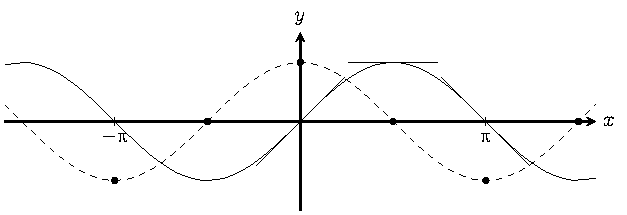
\includegraphics{basiccalculusandtrigonometry/sineandcosinerelation.pdf}
    \caption{The relation between sine (in black) and cosine (in dashed)}
    \label{fig:sine_cosine_relation}
\end{figure}

Let's start with the definition of the derivative given in \cref{eq:naive_definition_of_derivative},
\begin{equation}
    \odv*{\sin(x)}{x} = \lim_{h \appr 0}\frac{\sin(x + h) - \sin(x)}{h}.
\end{equation}
Using the sum of sines ($\sin(x + h) = \sin(x)\cos(h) + \cos(x)\sin(h)$),
\begin{align}
    \odv*{\sin(x)}{x} &= \lim_{h \appr 0}\frac{\sin(x)\cos(h) + \cos(x)\sin(h) - \sin(x)}{h}
    \intertext{When $h \appr 0$, $\cos(h) \appr 1$}
    &= \lim_{h \appr 0}\frac{\sin(x) + \cos(x)\sin(h) - \sin(x)}{h} \\
    &= \cos(x)\lim_{h \appr 0}\frac{\sin(h)}{h}.
    \intertext{For small angles, $\sin(h) \approx h$, therefore}
    &= \cos(x)\lim_{h \appr 0}\frac{h}{h} = \cos(x).
\end{align}
In conclusion, the derivative of sine is just the cosine just as we predicted with the graph.

Similarly, the derivative of cosine can also be found using the method of increments and using the sum of cosines formula $\cos(x + h) = \cos(x)\cos(h) - \sin(x)\sin(h)$
\begin{align}
	\odv*{\ab(\cos(x))}{x} &= \lim_{h \appr 0}\frac{\cos(x + h) - \cos(x)}{h} \\
						   &= \lim_{h \appr 0}\frac{\cos(x)\cos(h) - \sin(x)\sin(h) - \cos(x)}{h} \\
						   \intertext{When $h \appr 0$, $\cos(h) = 1$}
						   &= \lim_{h \appr 0}\frac{\cos(x) - \cos(x) - \sin(x)\sin(h)}{h} \\
						   &= \lim_{h \appr 0}\frac{-\sin(x)\sin(h)}{h}
						   \intertext{For small angles of $h$, $\sin(h) \approx h$}
						   &= \lim_{h \appr 0}\ab(-\sin(x)) = -\sin(x) 
\end{align}
I.e., the derivative of cosine is the negative of sine. From those two alone, we can form a set of formulas for differentiating sines and cosines:
\begin{equation}	
	\begin{aligned}
		\odv*{\ab(\sin(x))}{x} &= \cos(x) \\
		\odv*[order = 2]{\ab(\sin(x))}{x} &= \odv*{(\cos(x))}{x} = -\sin(x) \\
		\odv*[order = 3]{\ab(\sin(x))}{x} &= \odv*{(-\sin(x))}{x} = -\cos(x) \\
		\odv*[order = 4]{\ab(\sin(x))}{x} &= \odv*{(-\cos(x))}{x} = \sin(x)
	\end{aligned}
\end{equation}
We can see that the derivative of these two functions cycles in four: $\sin(x), \cos(x), -\sin(x), -\cos(x)$. From these alone, we can use the rules developed in \cref{sec:basic-derivatives-and-integrals}, e.g., the chain rule, power rule, etc., in order to find the derivative of other trigonometric functions.

\subsection{Derivative of other trigonometric functions}

Note that you can continue reading the next section straightaway. This section serves as a reference. But for those who are still interested, I'm glad to have you here. This is one of the places that uses the chain rule, product rule, and power rule a lot. It's a good exercise. Without further ado, let's start with the cosecant ($\csc(x) = \frac{1}{\sin(x)}$).
\begin{align}
	\odv*{\csc(x)}{x} &= \odv*{\frac{1}{\sin(x)}}{x} \\
						&= \odv*{\frac{1}{u}}{x} \cdot \odv{u}{u} && \textrm{Chain rule: $\sin(x) = u$} \\
						&= \odv*{u^{-1}}{u} \cdot \odv{u}{x} \\
						&= -1u^{-2}\cdot\odv*{\sin(x)}{x} && \textrm{Power rule, $u = \sin(x)$} \\
						&= -\frac{1}{\sin^2(x)}\cos(x) && \textrm{$\odv*{\sin(x)}{x} = \cos(x)$} \\
						&= -\csc(x)\cot(x) && \textrm{$\cot(x) = \frac{\cos(x)}{\sin(x)}$}.
\end{align}
And the secant function ($\sec(x) = \frac{1}{\cos(x)}$),
\begin{align}
	\odv*{\sec(x)}{x} &= \odv*{\ab(\frac{1}{\cos(x)})}{x} \\
					  &= \odv*{\ab(\frac{1}{u})}{x} \cdot \odv{u}{u} && \textrm{Chain rule: $\cos(x) = u$} \\
					  &= \odv*{u^{-1}}{u} \cdot \odv{u}{x} \\
					  &= -1u^{-2}\cdot\odv*{\cos(x)}{x} && \textrm{Power rule, $u = \cos(x)$}\\
					  &= -\frac{1}{\cos^{2}(x)}\ab(-\sin(x)) && \textrm{$\odv*{\cos(x)}{x} = -\sin(x)$} \\
					  &= \sec(x)\tan(x).
\end{align}

For the tangent function ($\tan(x) = \frac{\sin(x)}{\cos(x)}$), we use the product rule and the results from earlier
\begin{align}
	\odv*{\tan(x)}{x} &= \odv*{\frac{\sin(x)}{\cos(x)}}{x} \\
					  &= \odv*{\sin(x)\sec(x)}{x} \\
					  &= \sin(x)\odv*{\sec(x)}{x} + \sec(x)\odv*{\sin(x)}{x} \\
					  &= \sin(x)\sec(x)\tan(x) + \sec(x)\cos(x) \\
					  &= \sin(x)\frac{1}{\cos(x)}\frac{\sin(x)}{\cos(x)} + \frac{1}{\cos(x)}\cos(x) \\
					  &= \ab(\frac{\sin(x)}{\cos(x)})^2 + 1 = \tan^2(x) + 1 = \sec^2(x)
\end{align}
The Pythagorean identity is used in the last line to convert $1 + \tan^2(x)$ to $\sec^2(x)$. Of course, we cannot miss its reciprocal function: $\cot(x) = \frac{1}{\tan(x)}$.
\begin{align}
	\odv*{\cot(x)}{x} &= \odv*{\frac{1}{\tan(x)}}{x} \\
					  &= \odv*{\frac{\cos(x)}{\sin(x)}}{x} \\
					  &= \odv*{\cos(x)\csc(x)}{x} \\
					  &= \cos(x)\odv*{\csc(x)}{x} + \csc(x)\odv*{\cos(x)}{x} \\
					  &= \cos(x)\ab(-\csc(x)\cot(x)) + \csc(x)\ab(-\sin(x)) \\
					  &= -\cos(x)\frac{1}{\sin(x)}\frac{\cos(x)}{\sin(x)} - \frac{1}{\sin(x)}\sin(x) \\
					  &= -\ab(\cot^2(x) + 1) = -\csc^2(x),
\end{align}
where we've again used the Pythagorean identity $\cot^2(x) + 1 = -\csc^2(x)$.

Altogether, I've summarized all the derivatives of trigonometric functions into \cref{tab:derivative_trigonometric_functions}.
\begin{table}[ht]
	\begin{center}
		\begin{tabular}{C | L}
			f(x) & \odv*{f(x)}{x} \\
			\hline
			\sin(x) & \cos(x) \\
			\cos(x) & -\sin(x) \\
			\tan(x) & \sec^2(x) \\
			\hline
			\csc(x) & -\csc(x)\cot(x) \\
			\sec(x) & \sec(x)\tan(x) \\
			\cot(x) & -\csc^2(x)
		\end{tabular}
	\end{center}
	\caption{The derivatives of trigonometric functions}
	\label{tab:derivative_trigonometric_functions}
\end{table}

\section{Power series of trigonometric functions}

The approximation method that I'd be discussing are commonly taught to high schoolers with the name \textbf{small angle approximation}, i.e., for $\theta \appr 0$, \index{small angle approximation}
\begin{gather}
    \sin(\theta) \approx \tan(\theta) \approx \theta \mathand \cos(\theta) \approx 1 - \frac{\theta^2}{2}
\end{gather}
These approximations are very useful for calculating limits, e.g.,\footnote{Normally these limits are evaluated using the squeeze theorem. However, I don't want the mathematical intricacies to disrupt the flow of our journey right now. The full theorem will be discussed later at the end of the book.}
\begin{equation}
    \lim_{\theta \appr 0}\frac{\sin(n\theta)}{\theta} = \lim_{\theta \appr 0}\frac{n\theta}{\theta} = n.
\end{equation}
Here, I want to focus on where these approximations really comes from: the power series development of trigonometric functions.

\subsection{Power series of sine}

Assume that the sine function can be written as a power series
\begin{align}
	\sin(x) = s_0 + s_1x^1 + s_2x^2 + s_3x^3 + \dots
\end{align}
Because $\sin(0) = 0$,
\begin{align}
	\sin(0) &= s_0 + s_1(0)^1 + s_2(0)^2 + s_3(0)^3 + \dots \\
	s_0 = 0;
\end{align}
Because sine is an odd function, $\sin(-x) = -\sin(x)$; thus,
\begin{align}
	\begin{multlined}[b]
		s_1(-x)^1 + s_2(-x)^2 \\
		+ s_3(-x)^3 + s_4(-x)^4 + \dots
	\end{multlined} &=
	\begin{multlined}[t]
		-s_1x^1 - s_2x^2 \\
		- s_3x^3 - s_4x^4 + \dots 
	\end{multlined} \\
	\begin{multlined}[b]
		-s_1x^1 + s_2x^2 \\
		- s_3x^3 + s_4x^4 - \dots
	\end{multlined} &=
	\begin{multlined}[t]
		-s_1x^1 - s_2x^2 - \\
		s_3x^3 - s_4x^4 - \dots
	\end{multlined}
\end{align}
In the L.H.S., the sign alternates between negative and positive. In order for the L.H.S. to match the R.H.S., all the positive terms must vanish, leaving only the matching negative terms; therefore,
\begin{equation}
	\sin(x) = s_1x^1 + s_3x^3 + s_5x^5 + \dots.
\end{equation}
This is what we mean by \enquote{sine is an odd function}: there are only odd powers in its power series.

To find $s_1$, take the derivative of sine
\begin{equation}
	\odv*{\sin(x)}{x} = \cos(x) = s_1 + 3s_3x^2 + 5s_5x^4 + \dots,
\end{equation}
then substitute $x = 0$
\begin{align}
	\cos(0) = 1 &= s_1 + 3s_3(0)^2 + 5s_5(0)^4 + \dots \\
	1 &= s_1.
\end{align}
We can then take the derivative of sine again to get a recurrence relation.
\begin{align}
	\odv*[order = 2]{\sin(x)}{x} &= 3\cdot 2s_3x + 5\cdot 4s_5x^3 + 7\cdot 6s_7x^5 + \dots \\
	-\sin(x) &= \frac{3!}{1!}s_3x + \frac{5!}{3!}s_5x^3 + \frac{7!}{5!}s_7x^5 + \dots \\
	-s_1x - s_3x^3 - s_5x_5 - \dots &= \frac{3!}{1!}s_3x + \frac{5!}{3!}s_5x^3 + \frac{7!}{5!}s_7x^5 + \dots
\end{align}
By matching terms with the same order,
\begin{equation}	
	\begin{aligned}
		-s_1 &= \frac{3!}{1!}s_3x, \\
		-s_3 &= \frac{5!}{3!}s_5x, \\
		-s_5 &= \frac{7!}{5!}s_7x. \\
			 &\vdots
	\end{aligned}
\end{equation}
From $s_1 = 1$, we get that $s_3 = -\frac{1}{3!}$, $s_5 = -\frac{1}{5!}$, $s_7 = -\frac{1}{7!}$ etc. The negative sign alternates every term. We can then summarize the whole thing as
\begin{align}
	\sin(x) &= \sum_{n = 0}^{\infty}\frac{(-1)^{2n + 1}}{(2n + 1)!}x^{2n + 1} \\
			&= x - \frac{1}{3!}x^3 + \frac{1}{5!}x^5 - \frac{1}{7!}x^7 + \dots, \label{eq:sine-power-series}
\end{align}
which is the polynomial expansion of the sine function.

\subsection{Power series of cosine}

The power series of cosine can be developed using the same method as discussed earlier. But notice that the derivative of sine is cosine. Hence, we can just take the derivative of the sine's power series once to get the cosine's power series.
\begin{align}
	\odv*{\sin(x)}{x} &= \odv*{\ab(x - \frac{1}{3!}x^3 + \frac{1}{5!}x^5 - \frac{1}{7!}x^7)}{x} \\
	\cos(x) &= 1 - \frac{1}{2!}x^2 + \frac{1}{4!}x^4 - \frac{1}{6!}x^6 + \dots = \sum_{n = 0}^{\infty}\frac{(-1)^{2n}}{(2n)!}x^{2n}\label{eq:cosine-power-series}
\end{align}

\subsection{Power series of other trigonometric functions}

The same method could be used to find the power series expansion of secant, cosecant, tangent, etc. However, their power series doesn't actually represent the function because the other functions are all ratios of sine and cosines. To see what I mean, consider the behavior of the tangent function.

The tangent function is defined as $\tan\theta = \frac{\sin\theta}{\cos\theta}$. From this definition, $\tan\theta$ approaches infinity whenever $\cos\theta$ approaches zero, which is at $n\cpi$ where $n \in \mathbb{Z}$\footnote{$\mathbb{Z}$ is the set of integers}. As seen, there are infinitely many places in which the function approaches infinity. However, polynomials only have two infinities: at $x \appr \infty$, and $x \appr -\infty$; therefore, any polynomial expansion can't possibly represent the tangent function. The same logic also works for other trigonometric functions.

\subsection{Approximation of trigonometric functions}

One way a function can be approximated is by truncating its power series. To see why this is viable, consider the limit
\begin{align}
	\lim_{x \appr 0}\sin(x) = \lim_{x \appr 0}\ab(x - \frac{1}{3!}x^3 + \frac{1}{5!}x^5 - \frac{1}{7!}x^7 + \dots)
\end{align}
When $x \appr 0$, all the higher order degrees term vanishes; thus, 
\begin{gather}
	\lim_{x \appr 0}\sin(x) = x.
\end{gather}
It tells us that when $x \approx 0$, the sine function behaves like a linear function. Illustrated in \cref{fig:sine_small_angle},

\begin{figure}[ht]
	\centering
	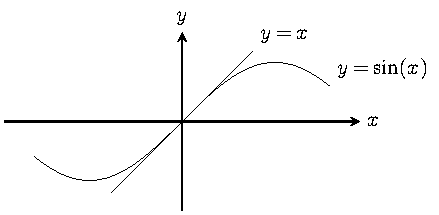
\includegraphics{basiccalculusandtrigonometry/sinesmallangle.pdf}
	\caption{Comparison of $y = \sin(x)$ and $y = x$ near $x = 0$}
	\label{fig:sine_small_angle}
\end{figure}
When $x$ gets larger, the higher order terms in the power series contributes more and more, so we need to include them. An excellent approximation for the sine function when $x \in [-\cpi, \cpi]$ is a truncation at the fifth term:
\begin{equation}
	\sin(x) \approx x - \frac{1}{3!}x^3 + \frac{1}{5!}x^5 - \frac{1}{7!}x^7 + \frac{1}{9!}x^9,
\end{equation}
plotted in \cref{fig:sine_approximation}. It is extremely accurate in that range.
\begin{figure}[t]
	\centering
	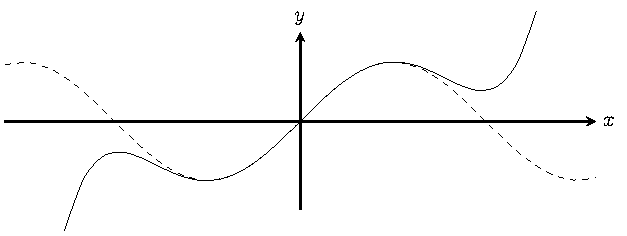
\includegraphics{basiccalculusandtrigonometry/sineapprox.pdf}
	\caption{An approximation of sine by truncating its power series at the fifth term.}
	\label{fig:sine_approximation}
\end{figure}
\begin{figure}[t]
	\centering
	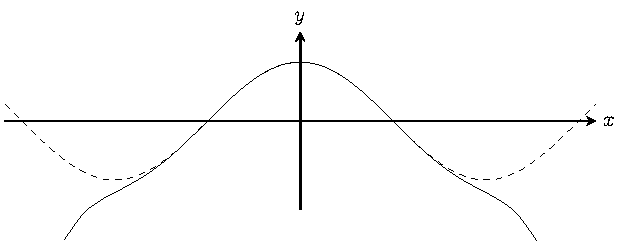
\includegraphics{basiccalculusandtrigonometry/cosineapprox.pdf}
	\caption{An approximation of cosine by truncating its power series at the fourth term}
	\label{fig:cosine_approximation}
\end{figure}
For cosine,
\begin{align}
	\lim_{x \appr 0}\cos(x) = \lim_{x \appr 0}\ab(1 - \frac{x^2}{2!} + \frac{x^4}{4!} - \dots) \approx 1 - \frac{x^2}{2!} \approx 1.
\end{align}
An acceptable approximation around zero is $1$ or $1 - \frac{x^2}{2}$. Similarly, an excellent approximation when $x \in [-\cpi, \cpi]$ is also a truncation at the fourth term:
\begin{equation}
	\cos(x) \approx 1 - \frac{1}{2!}x^2 + \frac{1}{4!}x^4 - \frac{1}{6!}x^6 
\end{equation}
plotted in \cref{fig:cosine_approximation}

\section{The harmonic oscillator}

\begin{figure}[ht]
	\centering
	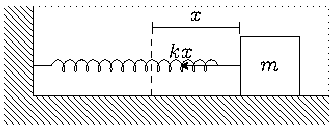
\includegraphics{basiccalculusandtrigonometry/harmonicoscillatorsetup.pdf}
	\caption{Setup of the harmonic oscillator}
	\label{fig:harmonic-oscillator-setup}
\end{figure}

Finally, we're ready to tackle our first oscillatory system: the harmonic oscillator. Illustrated in \cref{fig:harmonic-oscillator-setup}, consider a mass $m$ connected to a spring. The point that the spring is neither stretched or compressed is called the \textbf{equilibrium position}, drawn as the dashed line. The force that the spring acts on the mass depends on the displacement from the equilibrium position $x$:
\begin{equation}
	F = -kx,
\end{equation}
where $k$ is the stiffness of the spring. Higher $k$ represents a stiffer spring, and lower $k$ represents a looser spring. Newton's second law reads
\begin{align}
	-kx &= m\odv[ord = 2]{x}{t} \\
	-\frac{k}{m}x &= \odv[ord = 2]{x}{t}. \label{eq:spring-ord2}
\end{align}

We're interested in the solution of \cref{eq:spring-ord2} given an initial condition that at time $t = 0$, the mass is distance $A$ away from the equilibrium position, and it's released with zero initial velocity, i.e.,
\begin{equation}
	x(t = 0) = A \mathand \dot{x}(t = 0) = 0. \label{eq:spring-initial-condition}
\end{equation}

\subsection{Your first trigonometric substitution}

The equation that we got, \cref{eq:spring-ord2}, is an inseparable second order differential equation. It is extremely hard to work with. But by exploiting the chain rule, we can reduce it into a first order differential equation.
\begin{equation}
	\odv[ord = 2]{x}{t} = \odv*{\ab(\odv{x}{t})}{t} = \odv{\dot{x}}{t} = \odv{\dot{x}}{x}\odv{x}{t} = \dot{x}\odv{\dot{x}}{x}.
\end{equation}
\Cref{eq:spring-ord2} then becomes
\begin{align}
	-\frac{k}{m}x &= \dot{x}\odv{\dot{x}}{x} \\
	-\frac{k}{m}x\odif{x} &= \dot{x}\odif{\dot{x}} \\
	-\frac{k}{m}\int x\odif{x} &= \int\dot{x}\odif{\dot{x}} \\
	-\frac{k}{m}\frac{x^2}{2} &= \frac{\dot{x}^2}{2} + C \\
	-\frac{k}{m}x^2 &= \dot{x}^2 + C.
\end{align}
To find $C$, substitute in the initial condition \cref{eq:spring-initial-condition}.
\begin{align}
	-\frac{k}{m}(A)^2 &= (0)^2 + C \\
	C &= -\frac{k}{m}A^2. 
\end{align}
Thus,
\begin{align}
	-\frac{k}{m}x^2 &= \dot{x}^2 - \frac{k}{m}A^2 \\
	\dot{x}^2 &= \frac{k}{m}\ab(A^2 - x^2) \\
	\dot{x} &= \sqrt{\frac{k}{m}}\sqrt{A^2 - x^2}.
\end{align}
Because I'm too lazy to write square roots, let's use $\omega = \sqrt{\flatfrac{k}{m}}$; thus,
\begin{align}
	\dot{x} &= \omega\sqrt{A^2 - x^2} \\
	\odv{x}{t} &= \omega\sqrt{A^2 - x^2} \\
	\omega\odif{t} &= \frac{1}{\sqrt{A^2 - x^2}}\odif{x} \\
	\omega\int\odif{t} &= \int\frac{1}{\sqrt{A^2 - x^2}}\odif{x}. \label{eq:spring-ord1-d}
\end{align}
The L.H.S. directly evaluates to $\omega t$. But on the R.H.S., power rule substitution wouldn't work because there's a polynomial with degree two the root, but no terms with lower degree outside. If $u = A^2 - x^2$, we'd be going in loops. So how do we evaluate this?

The answer is, you can't do anything about it if we're going to use the methods so far. It's time for a new tool: \textbf{trigonometric substitution}.

The idea is very simple. We want to take advantage of the Pythagorean identity $1 - \sin^2\theta = \cos^2\theta$ to bring $A^2 - x^2$ out of the root. Substitute in $x = A\sin\theta$ and see what happens.
\begin{align}
	\int\frac{1}{\sqrt{A^2 - x^2}}\odif{x} &= \int\frac{1}{\sqrt{A^2 - A^2\sin^2\theta}}\odif{x} \\
										   &= \frac{1}{A}\int\frac{1}{\sqrt{1 - \sin^2\theta}}\odif{x} \\
										   &= \frac{1}{A}\int\frac{1}{\sqrt{\cos^2\theta}}\odif{x} = \frac{1}{A}\int\frac{1}{\cos\theta}\odif{x}
\end{align}
Taking care of the $\odif{x}$; if $x = A\sin\theta$, then
\begin{align}
	\odv{x}{\theta} &= A\odv{\sin\theta}{\theta} \\
	\odv{x}{\theta} &= A\cos\theta \\
	\odif{x} &= A\cos\theta\odif{\theta}.
\end{align}
Substituting back into the integral gives
\begin{equation}
	\frac{1}{A}\int\frac{1}{\cos\theta}\ab(A\cos\theta\odif{\theta}) = \int\odif{\theta} = \theta + C.
\end{equation}
Because $x = A\sin\theta$, $\theta = \arcsin\ab(\flatfrac{x}{A})$
\begin{equation}
	\int\frac{1}{\sqrt{A^2 - x^2}}\odif{x} = \arcsin\ab(\frac{x}{A}) + C.
\end{equation}
Thus, \cref{eq:spring-ord1-d} becomes
\begin{equation}
	\omega t = \arcsin\ab(\frac{x}{A}) + C.
\end{equation}
Then, substitute in the initial condition (\cref{eq:spring-initial-condition}) to find $C$:
\begin{align}
	\omega(0) &= \arcsin\ab(\frac{A}{A}) + C \\
	C &= \frac{\cpi}{2}.
\end{align}
Thus,
\begin{align}
	\omega t &= \arcsin\ab(\frac{x}{A}) + \frac{\cpi}{2} \\
	\arcsin\ab(\frac{x}{A}) &= \omega t + \frac{\cpi}{2} \\
	x &= A\sin\ab(\omega t + \frac{\cpi}{2}).
\end{align}
Since $\sin(\theta + \frac{\cpi}{2}) = \cos(\theta)$,
\begin{equation}
	x(t) = A\cos(\omega t) \label{eq:harmonic-oscillator-solution}
\end{equation}
which is the solution of the differential equation. It represents where the mass is relative to the equilibrium point over time. Taking the derivative of this once,
\begin{align}
	\dot{x}(t) &= A\odv{\cos(\omega t)}{t} \\
	\intertext{Let $u = \omega t$. By the chain rule,}
			&= A\odv{\cos(u)}{u} \times \odv{u}{t} \\
			&= -A\sin(u) \odv*{(\omega t)}{t} \\
			&= -\omega A\sin(\omega t), \label{eq:harmonic-oscillator-velocity}
\end{align}
we get the velocity as a function w.r.t. time. In a similar manner, taking the derivative of velocity again gives the acceleration
\begin{equation}
	\ddot{x} = \odv{\dot{x}}{t} = \odv{-A\omega\sin(\omega t)}{t} = -\omega^2A\sin(\omega t). \label{eq:harmonic-oscillator-acceleration}
\end{equation}

\subsection{The power series method}

Perhaps a faster method to solve \cref{eq:spring-ord2} is to just assume that the solution can be expanded in terms of power series
\begin{equation}
	x(t) = a_0 + a_1t + a_2t^2 + a_3t^3 + \dots. \label{eq:spring-series-x}
\end{equation}
Consequently,
\begin{gather}
	\dot{x}(t) = a_1 + 2a_2t + 3a_3t^2 + 4a^4t_3 + \dots \label{eq:spring-series-dot} \\
	\ddot{x}(t) = 2a_2 + 3\cdot 2a_3t + 4\cdot 3a_4t^2 + 5\cdot 4a_5t_3 + \dots \label{eq:spring-series-ddot}
\end{gather}
The initial condition given in \cref{eq:spring-initial-condition} ($x(t = 0) = A$, $\dot{x}(t = 0) = 0$) can then be used to find $a_0$ and $a_1$.
\begin{align}
	x(t = 0) &= a_0 + a_1(0) + a_2(0)^2 + a_3(0)^3 + \dots \\
	a_0 &= A
\end{align}
and from \cref{eq:spring-series-dot},
\begin{align}
	\dot{x}(t = 0) &= a_1 + 2a_2(0) + 3a_3(0)^2 + 4a_4(0)^3 + \dots \\
	a_1 &= 0
\end{align}
The rest of the terms can be found by using the differential equation itself. First, rearrange the equation into
\begin{equation}
	\odv[ord = 2]{x}{t} + \omega^2x = 0.
\end{equation}
Then, substitute in \cref{eq:spring-series-x,eq:spring-series-ddot}
\begin{align}
	0 &= \odv[ord = 2]{x}{t} + \omega^2x\\
	0 &= \begin{multlined}[t]
		\ab(2a_2 + 3\cdot 2a_3t + 4\cdot 3a_4t^2 + 5\cdot 4a_5t^3 + 6\cdot 5a_6t^4 + 6\cdot 7a_7t^5 + \dots) \\ + \ab(\omega^2A + a_2\omega^2t^2 + a_3\omega^2t^3 + a_4\omega^2t^4 + a_5\omega^2t^5\dots) \nonumber
	\end{multlined} \\
	0 &= \begin{aligned}[t]
		&\ab(2a_2 + \omega^2A) \\
		& +(3 \cdot 2a_3)t \\
		& +(4\cdot 3a_4 + \omega^2a_2)t^2 \\
		& +(5\cdot 4a_5 + \omega^2a_3)t^3 \\
		& +(6\cdot 5a_6 + \omega^2a_4)t^4 \\
		& +(7\cdot 6a_7 + \omega^2a_5)t^5 + \dots\\
	\end{aligned}
\end{align}
For the R.H.S. to be $0$, all terms must vanish; thus, we get an infinite series of equations to be evaluated
\begin{equation}
	\begin{aligned}
		0 &= \ab(2a_2 + \omega^2A) \\
		0 &= (3 \cdot 2a_3) \\
		0 &= (4\cdot 3a_4 + \omega^2a_2) \\
		0 &= (5\cdot 4a_5 + \omega^2a_3) \\
		0 &= (6\cdot 5a_6 + \omega^2a_4) \\
		0 &= (7\cdot 6a_7 + \omega^2a_5) \\
		  &\vdots
	\end{aligned}
\end{equation}
Starting from the second one: $0 = 3 \cdot 2a_3$ means that $a_3 = 0$. This eliminates every term that includes $a_3$. The fourth equation says $5\cdot 4a_5 + \omega^2a_3 = 0$, thus $a_5 = 0$. This pattern continues, eliminating every odd terms in the series. We're then left with
\begin{equation}
	\begin{aligned}
		0 &= 2a_2 + \omega^2A \\
		0 &= 4\cdot 3a_4 + \omega^2a_2 \\
		0 &= 6\cdot 5a_6 + \omega^2a_4 \\
		0 &= 8\cdot 7a_8 + \omega^2a_6 \\
		  &\vdots
	\end{aligned}
\end{equation}
Starting from the first one, we get $a_2 = -\frac{\omega^2}{2}A$. The second equation gives $a_4 = \frac{\omega^4}{4!}A$. The third gives $a_6 = \frac{\omega^6}{6!}A$. This pattern of $a_{2n} = \frac{\omega^{2n}}{2n}A$ continues on forever. The power series expansion for $x(t)$ gives
\begin{align}
	x(t) &= a_0 + \cancelto{0}{a_1} + a_2t^2 + \cancelto{0}{a_3}t^3 + a_4t^4 + \cancelto{0}{a_5}t^5 + a_6t^6 + \dots \\
		 &= A + A\frac{\omega^{2}}{2!}t^2 + A\frac{\omega^{4}}{4!}t^4 + A\frac{\omega^{6}}{6!}t^6 + \dots \\
		 &= A\ab(\frac{(\omega t)^2}{2!} + \frac{(\omega t)^4}{4!} + \frac{(\omega t)^6}{6!} + \dots)
\end{align}
Looks familiar yet? \emph{This}, the result that we got is exactly the power series expansion for cosine (\cref{eq:cosine-power-series}); thus,
\begin{equation}
	x(t) = A\cos(\omega t).
\end{equation}

\subsection{Physical aspects of the harmonic oscillator}

Now that we have solved the harmonic oscillator, let's bring our attention to the qualitative description of the system.

The mass is released with zero velocity at $x = A$. As the spring tries to restore its equilibrium, it accelerates the mass towards the equilibrium position. The further the mass is from the equilibrium, the stronger the spring pulls. Initially, the spring pulls very hard on the mass, causing it to accumulate much velocity. But as it approaches the equilibrium position, the spring's force diminishes and there is barely any force left to stop the mass, so it overshoots the other side, compressing the spring. This oscillatory cycle continues on forever. Intuitively, we can predict that the mass will have the highest velocity and lowest acceleration as it directly passes through the equilibrium; and, lowest velocity and highest acceleration when the spring is fully stretched or compressed. But does the mathematics agree with this?

In \cref{fig:harmonic-oscillator-position-velocity}, the position function (\cref{eq:harmonic-oscillator-solution}) is plotted in thick lines, and the velocity function (\cref{eq:harmonic-oscillator-velocity}) are plotted in dashed lines.

The furthest point that a mass could be from a spring is at $x = \pm A$. Mathematically, this represents the local maxima and minima of the function, which can be obtained by taking the first derivative and setting it to zero (\cref{sec:minima-and-maxima}). The derivative of the position w.r.t. time is just the velocity (\cref{eq:harmonic-oscillator-velocity}), and it reaches zero whenever $\sin(\omega t)$ is zero
\begin{align}
	\sin(\omega t) &= 0 \\
	\omega t &= \arcsin(0) + 2n\cpi && n \in \mathbb{Z}\\
	t &= \frac{(2n + 1)\cpi}{\omega}. \label{eq:harmonic-oscillator-max-position}
\end{align}
Another way to derive this fact is to just notice that the range of the cosine function only extends from $-1$ to $1$; therefore, the highest that $A\cos(\omega t)$ can go is just $A$. So, another equation that we can form is
\begin{align}
	\cos(\omega t) = 1 \\
	\omega t = \arccos(1) + 2n\cpi && n \in \mathbb{Z} \\
	t = \frac{(2n + 1)\cpi}{\omega},
\end{align}
which has the same solution as $\sin(\omega t) = 0$.

\begin{figure}[ht]
	\centering
	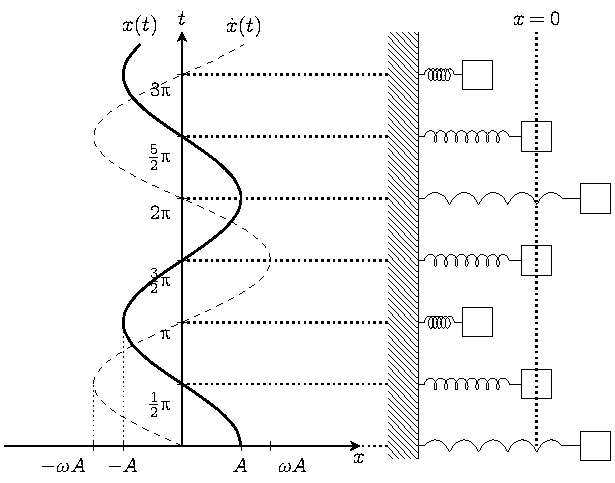
\includegraphics{basiccalculusandtrigonometry/harmonic-oscillator-position-velocity.pdf}
	\caption{The trajectory of a mass in the harmonic oscillator system. (Left) The position is plotted in thick lines, and the velocity, in dotted lines. (Right) Depiction of an oscillating mass, according to the solution of the differential equation.}
	\label{fig:harmonic-oscillator-position-velocity}
\end{figure}

The time that the mass goes through the equilibrium position can be found by just setting $A\cos(\omega t)$ to zero
\begin{align}
	A\cos(\omega t) &= 0 \\
	\omega t &= \arccos(0) + 2n\cpi && n \in \mathbb{Z}\\
	t &= \frac{2n\cpi}{\omega} \label{eq:harmonic-oscillator-zero-position}
\end{align}

Since the velocity function (\cref{eq:harmonic-oscillator-velocity}) is a sine function, it must oscillates $\cpi$ radians off-phase relative to the position function. Therefore, 
\begin{enumerate}
	\item Whenever the mass is furthest away from the equilibrium, the velocity is zero
	\item Whenever the mass is directly passing through the equilibrium, the velocity reaches its maximum at $\pm\omega A$
\end{enumerate}
The first fact can be easily verified by setting the velocity function, $-\omega A\sin(\omega t)$ equals to zero
\begin{align}
	-\omega A\sin(\omega t) &= 0 \\
	\omega t &= \arcsin(0) + 2n\cpi \\
	t &= \frac{(2n + 1)}{\omega},
\end{align}
which directly matches with the point of furthest position (\cref{eq:harmonic-oscillator-max-position}). The second one can be verified by taking the derivative of velocity, which is just the acceleration, found in \cref{eq:harmonic-oscillator-acceleration}. Setting that equals to zero yields
\begin{align}
	-\omega^2A\cos(\omega t) &= 0 \\
	\omega t &= \arccos(0) + 2n\cpi \\
	t &= \frac{2n\cpi}{\omega},
\end{align}
which matches our result from \cref{eq:harmonic-oscillator-zero-position}.

The acceleration function is again, a cosine function that's in phase with the position. Therefore, the local minima and maxima from the position function must match. We can quickly conclude that the acceleration is at its highest at $t = \frac{2n\cpi}{\omega}$, and is zero at $\frac{(2n + 1)\cpi}{\omega}$.

You would think that we have completed the physical aspects of the harmonic oscillator. But there is something I left over: the $\omega$ term. Since the beginning, I have assigned $\omega = \sqrt{\frac{k}{m}}$ as a notational trick for convenience. Is there any real physical meaning behind $\omega$?

If you don't know much about units, it's fine if you skip these paragraphs straightaway. But one clue that suggests the physical meaning of $\omega$ is its unit. Since $\omega = \sqrt{\frac{k}{m}}$, we have to analyse the units of its components separately. $k$ is a spring stiffness constant which is got from
\begin{equation}
	F = -kx \mathor k = -\frac{F}{x}.
\end{equation}
$F$ is the unit of force (Newton $\unit{\newton}$), which is just $\unit{\kilogram}\frac{\unit{\meter}}{\unit{\second^2}}$), and $x$, the units of distance (Meters $\unit{\meter}$); therefore, $k$ is the unit of
\begin{equation}
	\frac{\unit{\kilogram}\frac{\unit{\meter}}{\unit{\second^2}}}{\unit{\meter}} = \frac{\unit{\kilogram}}{\unit{\second^2}}.
\end{equation}
And since $m$ has the unit of kilogram ($\unit{\kilogram}$), $\omega$ which is $\sqrt{\frac{k}{m}}$ has the unit of
\begin{equation}
	\sqrt{\frac{\frac{\unit{\kilogram}}{\unit{\second^2}}}{\unit{\kilogram}}} = \sqrt{\frac{1}{\unit{\second^2}}} = \frac{1}{\unit{\second}}
\end{equation}
Funnily enough, this is the unit of Hertz, ($\frac{1}{\unit{\second}} = \unit{\hertz}$) which describes a frequencies. But it cannot possibly be just a unit of frequency because the solution of the differential equation says so.

The solution of our equation is $x(t) = A\cos(\omega t)$. If $\omega$ is really a unit of Hertz, then $\omega t$ would have no units, which contradicts that the cosine function either accepts radians ($\unit{\radian}$), or degrees ($\unit{\deg}$). But these are units that are dimensionless, meaning that we can just multiply it into $\omega$; therefore, $\omega$ must have the unit of $\unit{\radian\per\second}$, which is the unit of angular frequencies.

The conclusion that $\omega$ is the angular frequencies can also be directly deducted from the solution of the equation. From both of \cref{eq:harmonic-oscillator-max-position} and \cref{eq:harmonic-oscillator-zero-position}, the time between each maximum and minima point is divided by $\omega$. If $\omega$ is very high, then the time between the maximum and minimum is decreased. If it's low, then the time is increased. Therefore, $\omega$ is directly associated to the natural frequency of the system. The more $\omega$ is, the more frequent the oscillator oscillates.

Another way $\omega$ can be interpretted is by looking at the expression of $\omega$ itself: $\sqrt{\frac{k}{m}}$. The spring stiffness constant $k$ is on the top, so it means the stiffer the spring, the higher omega is. A stiffer spring would allow the spring to pull the mass faster; thus, increasing the frequencies. The mass $m$ is on the bottom: the larger the mass, the lower the omega. That just means a more massive block is harder for the spring to move; therefore, the mass will travel slower, decreasing the frequencies.

\subsection{Solution for other initial conditions. A trick with simplifying inverse trigonometric functions.}

Now, let's see what happens if the initial condition is changed from $x(t = 0) = A$, and $v(t = 0) = 0$, to
\begin{equation}
	x(t = 0) = X \mathand v(t = 0) = V.
\end{equation}
Since it's the same system but just under a different initial condition, the differential equation stays exactly the same
\begin{equation}
	\odv[ord = 2]{x}{t} + \omega^2x = 0,
\end{equation}
where $\omega = \sqrt{\flatfrac{k}{m}}$ for the same notational reason. In a similar manner, use the chain rule on the second derivative to reduce it down to a first order differential equation:
\begin{align}
	\dot{x}\odv{\dot{x}}{x} &= -\omega^2x \\
	\dot{x}^2 &= -\omega^2x^2 + C.
\end{align}
To find the initial condition, set $t = 0$ and substitute $x(t = 0) = X$ and $v(t = 0) = V$.
\begin{align}
	V^2 &= -\omega^2(X)^2 + C \\
	C &= \omega^2X^2 + V^2.
\end{align}
Since the form is quite complex, let's call this $C_1$, and substitute it in later when the differential equation is fully solved. So,
\begin{align}
	\dot{x}^2 &= -\omega^2x^2 + C_1 \\
	\odv{x}{t} &= \sqrt{-\omega^2x^2 + C_1} \\
	\int\odif{t} &= \int\frac{1}{\sqrt{C_1 - \omega^2x^2}}\odif{x} \\
	t &= \int\frac{1}{\frac{1}{\omega}\sqrt{\ab(\flatfrac{\sqrt{C_1}}{\omega})^2 - x^2}}\odif{x} \\
	t &= \omega\int\frac{1}{\sqrt{\ab(\flatfrac{\sqrt{C_1}}{\omega})^2 - x^2}}\odif{x}
\end{align}
Since $C_1$ is always positive due to its term all being squared. The same trigonometric substitution can be used to obtain
\begin{align}
	t = \omega\arcsin\ab(\frac{x}{\flatfrac{\sqrt{C_1}}{\omega}}) + C_2
\end{align}
Then, set $t = 0$, and substitute $x(t = 0) = X$ to find $C_2$.
\begin{align}
	0 &= \omega\arcsin\ab(\frac{\omega X}{\sqrt{C_1}}) + C_2 \\
	C_2 &= -\omega\arcsin\ab(\frac{\omega X}{\sqrt{\omega^2X^2 + V^2}})
\end{align}


\subsection{The ansatz method}

\section{Damped harmonic oscillator}

\section{Substitution to eliminate trigonometric functions}

\section{Circles and ellipses}

\subsection{Perimeter}

\subsection{Areas of circle. A funny way to approximate pi.}

\section{Volume of revolutions}
